%Preámbulo
\documentclass[a4paper]{article}
\usepackage[spanish]{babel}
\usepackage[utf8]{inputenc}
\usepackage[pdftex]{graphicx}
\parindent=0.3cm %Modificar el tamaño de la sangría
\usepackage{float} %Movimiento de tablas y gráficos
\usepackage[lmargin=2.5cm,rmargin=2.5cm,top=2.5cm,bottom=2.5cm]{geometry} %Márgenes

%Encabezado
\usepackage{fancyhdr}
\pagestyle{fancy}
\fancyhead{} %Elimina el texto predeterminado del encabezado fancy
\fancyhead[C]{La muda en los artrópodos} %Texto del encabezado
\renewcommand{\headrulewidth}{0.25pt} %Grosor de la línea

%Pie de página
\fancyfoot{} %Elimina el texto predeterminado del pie de página
\fancyfoot[R]{\thepage} %Comando para la numeración de página
\fancyfoot[L]{Jorge Garrido Bautista}

%COMIENZO DEL DOCUMENTO
\begin{document}

%Página inicial - título del artículo
\begin{titlepage}
\begin{center}
\vspace*{5\baselineskip} %Espacio vertical
{\LARGE \textbf{Análisis de expresión de genes de desarrollo larvario en el camarón Palaemon serratus (Pennant, 1777)}}
\vspace*{5\baselineskip}
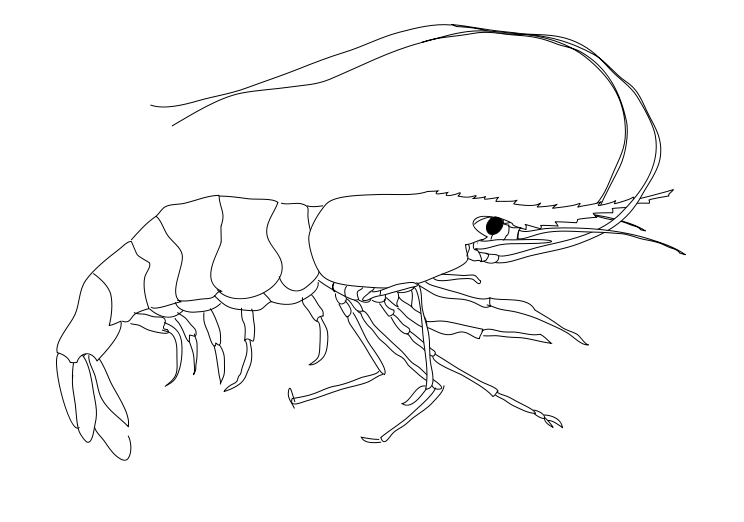
\includegraphics[scale=0.4]{Figura portada (Wikipedia).png}
\vfill %Este comando rellena con huecos vacíos el espacio entre la imagen y el último texto
{\large JORGE GARRIDO BAUTISTA}\\
Universidade da Coruña\\
Máster en Biología Molecular, Celular y Genética
\end{center}
\end{titlepage}

\section{Introducción}
\subsection{La muda en artrópodos}
\subsection{Regulación endocrina de la muda}

\end{document}
